\documentclass{article}
\usepackage[utf8]{inputenc}
\usepackage{graphicx}
\usepackage[spanish]{babel}


\begin{document}

\begin{figure}[t!]

\includegraphics[scale=0.3]{logo_udp.PNG}
\label{fig:udplogo}
\end{figure}

\title{\textbf{{Laboratorio 1 \\ Cableado Estructurado \vspace{10cm}}}}
\author{\hspace{8cm} Vicente Henriquez \\ \hspace{8cm} Franco Montenegro}
\date{\hspace{8cm} 30 de agosto, 2017}
\maketitle

\newpage
\tableofcontents

\newpage
\section{Introducción\vspace{0.5cm}}
Luego de que la CCIA le solicitara a la EIA crear una norma que rigiera el estándar para el cableado estructurado, aparece la norma EIA-568B, la cual será estudiada en este laboratorio, dicha norma tiene dos formas para colocar los cables en el conector RJ-45, las cuales son T568A y T568B.
La idea principal es aprender como armar un cable UTP de categoría 5 y su funcionamiento, con las diferentes herramientas facilitadas para este proceso se busca el poder completar la forma directa(T568A-T568A) y la forma cruzada(T568A-T568B) de los cables para la implementación de una área de red local (LAN)
\newpage
\section{Desarrollo \vspace{0.5cm}}
\subsection{Armado del cable\vspace{0.3cm}}
Con el objetivo de armar el cable UTP de la manera más perfecta y profesional posible se nos facilita de una crimpeadora, 3 conectores RJ45 y un cable UTP Cat.5 como se ven en la Figura \ref{fig:material}.

\begin{figure}[h!]
\centering
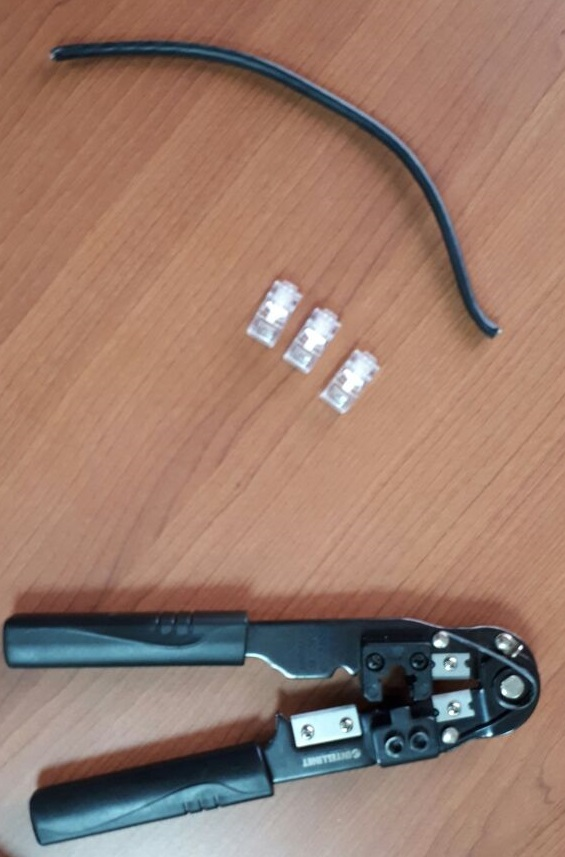
\includegraphics[scale=0.2 , angle = 90]{materiales.jpg}
\caption{Materiales}
\label{fig:material}
\end{figure}

Primero se armó un cable de tipo cruzado, es decir, que por un lado tendríamos T568A y por el otro extremo T568B dando como resultado lo que se aprecia en la Figura \ref{fig:cruz}

\begin{figure}[h!]
\centering
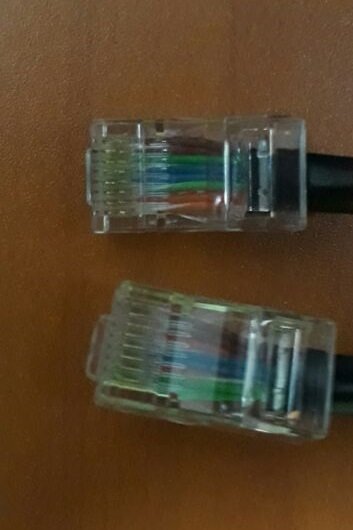
\includegraphics[scale=0.3 , angle = -90]{Cruzado.jpg}
\caption{Conexión cruzada}
\label{fig:cruz}
\end{figure}

Luego se le cortó una de las puntas al cable antes armado para realizar la segunda parte de la activida: convertir el cable a uno de tipo Directo (Figura \ref{fig:direc})

\begin{figure}[h!]
\centering
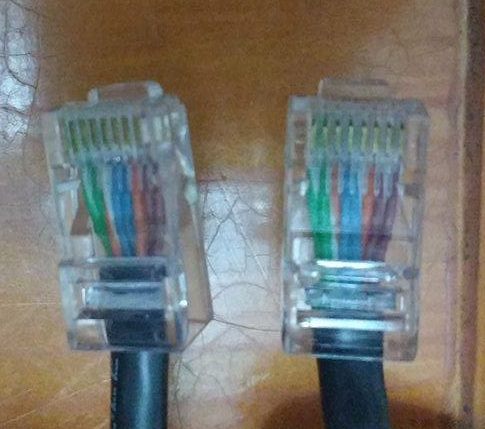
\includegraphics[scale=0.3 ,width=4cm, height=2cm]{directo.jpg}
\caption{Conexión Directa}
\label{fig:direc}
\end{figure}
\newpage

\subsection{Preguntas\vspace{0.3cm}}

\begin{enumerate}
\item¿Cuál es la diferencia entre EIA-568A y EIA-568B? Explique. \\
\newline La única diferencia entre T568A y T568B es que los pares 2 y 3 están alternados. Ambos estándares conectan los cables "directamente", es decir, los pines 1 a 8 de cada extremo se conectan con los pines 1 a 8, respectivamente, en el otro. Asimismo, los mismos pares de cables están emparejados en ambos estándares: pines 1-2, 3- 6, 4-5 y 7-8. Y aunque muchos cables implementan pequeñas diferencias eléctricas entre cables, estos efectos son inapreciables, de manera que los cables que utilicen cualquier estándar son intercambiables.\\

\item¿Cuáles son los tipos de cables UTP existentes? ¿En qué se diferencian? Puede expresarlo en una tabla o en palabras.\\
\begin{itemize} 
\item \textbf{ Categoría 1:}
Es el más adecuado para las comunicaciones telefónicas. No es adecuado para transmitir datos o para trabajarlos en una red. Se utiliza sobre todo en instalaciones de cableado.

\item \textbf{ Categoría 2:}
Es capaz de transmitir datos de hasta 4 Mbps. Se usó en las redes ARCnet (arco de red) y Token Ring (configuración de anillo) hace algún tiempo. El CAT 2 al igual que el CAT 1, no es adecuado para la transmisión de datos en una red.

\item \textbf{ Categoría 3:}
Es un par trenzado, sin blindar, capaz de llevar a la creación de redes 100BASE-T y puede ayudar a la transmisión de datos de hasta 16MHz con una velocidad de hasta 10 Mbps. No se recomienda su uso con las instalaciones nuevas de redes.

\item \textbf{ Categoría 4:}
Es un par trenzado sin blindar que soporta transmisiones de hasta 20MHz. Es confiable para la transmisión de datos por encima del CAT 3 y puede transmitir datos a una velocidad de 16 Mbps. Se utiliza sobre todo en las redes Token Ring.

\item \textbf{Categoría 5:}
Ayuda a la transmisión de hasta 100 MHz con velocidades de hasta 1000 Mbps. Es un cable UTP muy común y adecuado para el rendimiento 100BASE T. Se puede utilizar para redes ATM, 1000BASE T, 10BASE T, 100BASE T y token ring. Estos cables se utilizan para la conexión de computadoras conectadas a redes de área local.

\item \textbf{Categoría 5e:}
El cable categoría 5e o CAT 5e, es una versión mejorada sobre el de nivel 5. Sus características son similares al CAT 5 y es compatible con transmisión de hasta 10MHz. Es más adecuado para operaciones con Gigabit Ethernet y es una excelente opción para red 1000BASE T.

\item \textbf{Categoría 6:}
Es una propuesta de par trenzado sin blindar que puede soportar hasta 250 MHz de transmisión. Se trata de la sexta generación del cable Ethernet. Este cable con alambres de cobre puede soportar velocidades de 1 GB. CAT 6 es compatible con el CAT 5e, CAT 6 y CAT 3. Es adecuado para redes 1000BASE T, 100BASE T y 10BASE T y posee estrictas reglas acerca del ruido del sistema y la diafonía.

\item \textbf{Categoría 7:}
Es otro proyecto de norma que admite la transmisión de hasta 600MHz. CAT 7 es un estándar Ethernet de cable de cobre 10G que mide más de 100 metros. Es compatible con CAT 5 y CAT 6 y tiene reglas más estrictas que CAT 6 sobre el ruido del sistema y la diafonía.
\end{itemize}

\item¿De qué se encarga la CCIA?\\
\newline La CCIA es una organización internacional que se dedica a la innovación y mejoramiento a la información y comunicaciones por parte de la sociedad,promueve el mercado, sistemas y redes abiertas, para una abierta competencia en computación, telecomunicación e industrias de internet.
\item¿Cuál es la diferencia entre los cables UTP y el cable de fibra óptica?\\
\newline Los cables UTP consisten en un par de cables de cobre aislados que son enrollados para evitar el efecto antena y, dependiendo de sus números de trenzas por unidad de longitud, se clasifican en categorías (1,2,3,4,5,6,7). A mayor numero de trenzas se reduce la interferencia y se obtiene mayor velocidad de transferencia.
Actualmente estos cables, que tienen un bajo costo y son fáciles de instalar, alcanzan los 10 Gbps(Cat 6).
Los de fibra, por otra parte, están hechos de un hilo muy fino de material transparente, vidrio o materiales plásticos por el que se envían pulsos de luz que representan los datos a transmitir, pulsos que llegan hasta los 100 haces de luz a 10 Gb/s y una tasa de transmisión de 10 Tb/s. Estos cables son inmunes al electromagnetismo y son más ligeros que los cables de cobre pero los costos son mucho mayores con respecto a los UTP.\\

\item¿Cuál es la base sobre la cual funciona el cable UTP?\\
\newline Un cable UTP es un cable de telecomunicaciones que se compone de varios conductores de cobre, recubiertos por un material de plástico aislante. Estos conductores están ordenados de a pares y trenzados para disminuir la incidencia de las interferencias externas o proveniente de los otros cables, la cantidad de pares trenzados es de 4.Con esto y los conectores RJ-45 macho componemos en su totalidad el cable, y este se introduce en un conector RJ-45 hembra.
\end{enumerate}
\newpage

\section{Conclusión \vspace{0.5cm}}
Si bien la complejidad del armado de este tipo de cables no es mayor, hay que ser sumamente meticuloso en este proceso puesto que los materiales en sí son fáciles de deteriorar, es decir, que durante la construcción (por ejemplo) no se puede doblar agresivamente el cable o cortar irresponsablemente, los conectores se pueden romper si no son apretados por la crimpeadora correctamente, no se puede estimar el corte en las puntas de los cables sin pensar, hay que fijarse que los pines lleguen al final y así con una lista de detalles más pero que, de no obviar dicha lista, nos permitirá realizar una correcta implementación de nuestra red de área local.


\end{document}
